\documentclass[../main.tex]{subfiles}
\begin{document}
    \subsection{Testowanie}
    Testowanie oprogramowania to \textbf{wykonywanie kodu dla pewnych kombinacji} danych wejściowych i
    stanów w celu wykrycia błędów.

    \textbf{Udany test - wykrycie błędu.} Efektywność testu - zdolność do znajdywania błędów.

    Testowanie $+$ statyczna weryfikacja $=$ \textbf{pełne pokrycie dla weryfikacji i walidacji}.

    Testowanie jest \textbf{jedyną techniką walidacji dla wymagań niefunkcjonalnych}.

    \begin{table}[H]
        \begin{center}
            \begin{tabular}{ c p{8cm} }
                \raisebox{-\totalheight}{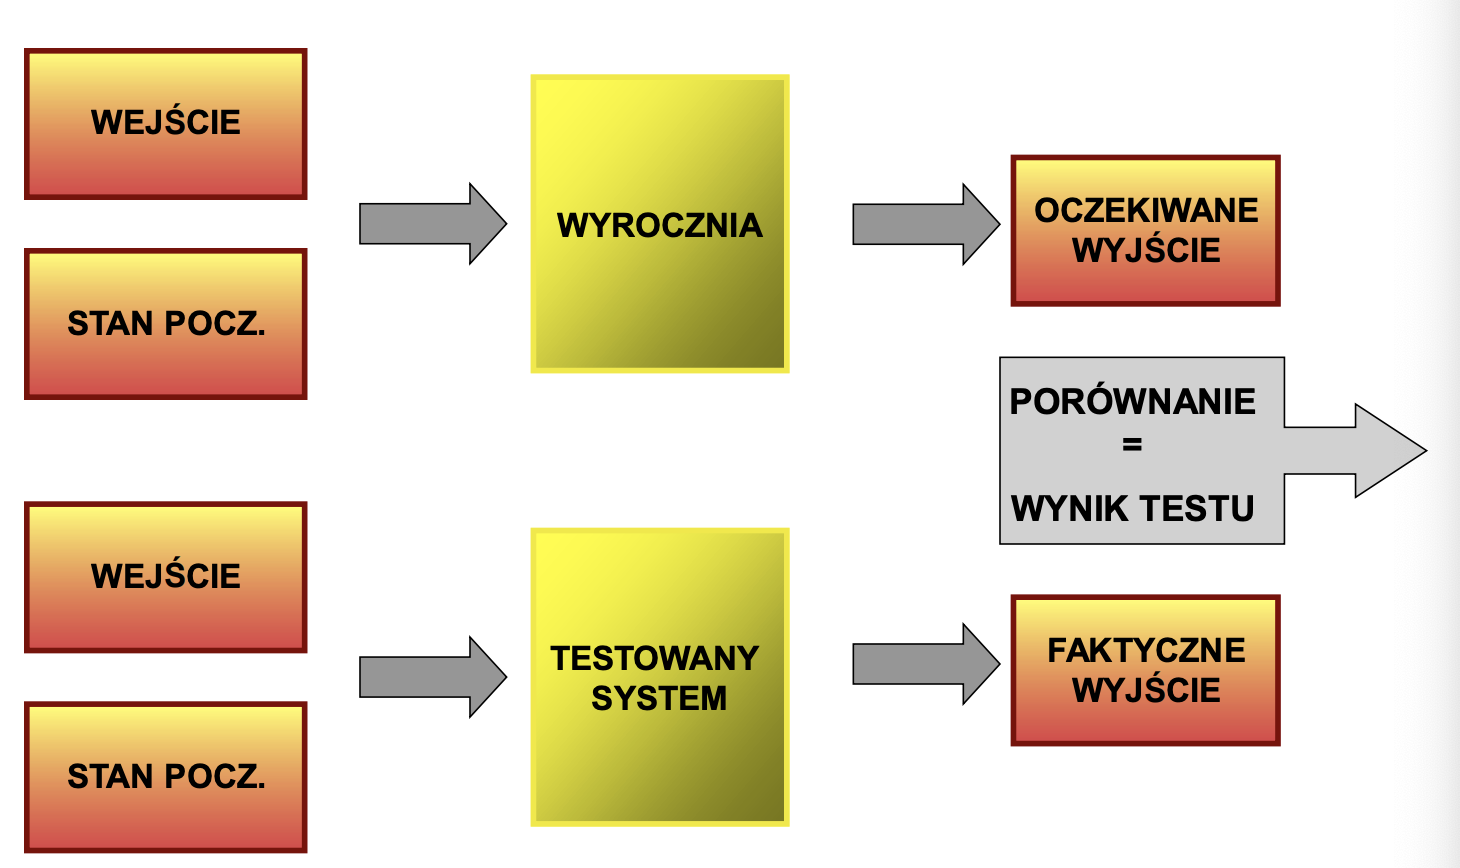
\includegraphics[width=0.5\textwidth]{testy.png}}
                &
                \textbf{Planowanie testów}
                \begin{itemize}
                    \item im wcześniej rozpoczniemy tym lepiej;
                    \item statyczna weryfikacja czy testowanie?
                    \item zasada Patero;
                    \item definiowanie standardów dla testowania;
                \end{itemize}

                \textbf{Dokument planu testów}
                \begin{itemize}
                    \item Proces testowania
                    \item Śledzenie wymagań
                    \item Testowane elementy
                    \item Harmonogram testów
                    \item Procedury nagrywania testów
                    \item Wymagania odnośnie sprzętu i oprogramowania
                    \item Ograniczenia
                \end{itemize}

                \\
            \end{tabular}
        \end{center}
    \end{table}



    \subsubsection{Aksjomaty testowania}


    \begin{table}[H]
        \begin{center}
            \begin{tabular}{ c c }
                \raisebox{-\totalheight}{\includegraphics[width=0.5\textwidth]{t_aks1.png}}
                &
                \raisebox{-\totalheight}{\includegraphics[width=0.5\textwidth]{t_aks2.png}}
                \\
            \end{tabular}
        \end{center}
    \end{table}




    Pokrycie kodu
    \begin{itemize}
        \item \textbf{Pokrycie instrukcji}: sprawdzana jest każda instrukcja,
        \item \textbf{Pokrycie gałęzi}: odwiedzamy każda gałąź; instrukcja warunkowa musi być raz spełniona a raz fałszywa.
    \end{itemize}


    \subsubsection{Rodzaje testów}

    \textbf{Rodzaje testów}
    \begin{itemize}
        \item jednostkowe
        \item integracyjne
        \item systemowe
        \item akceptacyjne
    \end{itemize}


    \textbf{Rodzaje testów (faza pielęgnacji)}
    \begin{itemize}
        \item regresyjne
        \item smoke test
    \end{itemize}


    \textbf{Techniki testowania}
    \begin{itemize}
        \item white box
        \item black box
    \end{itemize}


    \subsubsection{Automatyzacja testowania}
    \begin{itemize}
        \item \textbf{Bardzo istotny wybór wariantów testów}
        \item Automatyzacja testów znacznie różni się od testowania.
        \item Bywa bardzo kosztowna, droższa nawet od ręcznego wykonania testów.
    \end{itemize}

    \textbf{Obietnice automatyzacji testowania}
    \begin{itemize}
        \item Zwiększenie testowania (przypadki testowe uruchamiane w minutach)
        \item Zmniejszenie kosztu testowania aż do 80% wysiłku ręcznegotestowania
        \item Lepszej jakości oprogramowanie wyprodukowane szybciej
    \end{itemize}

    \textbf{Ocena jakości wariantu testu}

    \begin{table}[H]
        \begin{center}
            \begin{tabular}{ c p{8cm} }
                \raisebox{-\totalheight}{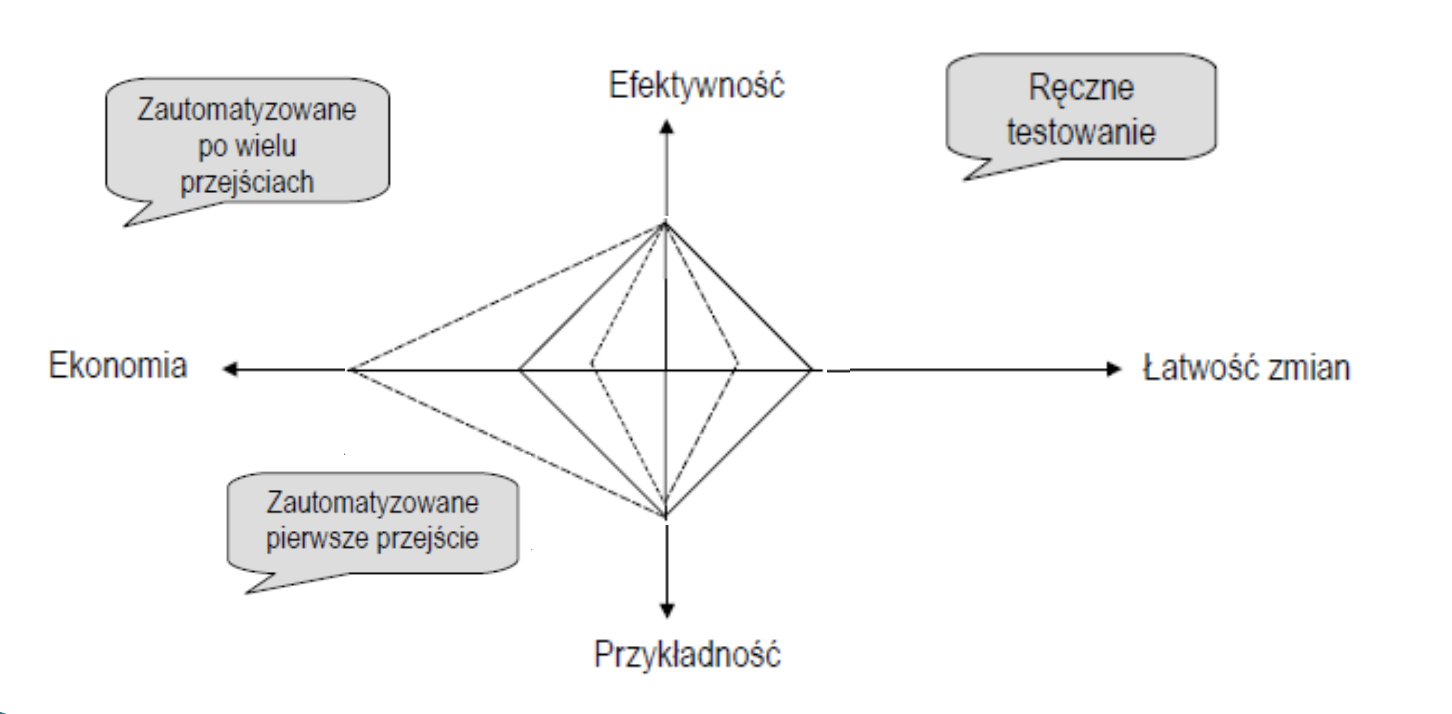
\includegraphics[width=0.5\textwidth]{jakosc_testu.png}}
                &
                \textbf{Czynności w ramach testowania}
                \begin{itemize}
                    \item Identyfikacja warunków testu
                    \item Zaprojektowanie przypadków testowych
                    \item Zbudowanie przypadków testowych
                    \item Uruchomienie przypadków testowych
                    \item Porównanie uzyskanych wyników z oczekiwanymi
                \end{itemize}
                \textbf{Które z czynności najlepiej zautomatyzować?}
                \\
            \end{tabular}
        \end{center}
    \end{table}


    \subsection{Kontrola jakości}


    \begin{itemize}
        \item \textbf{Jakość} - zgodność z wymaganiami,
        \item \textbf{Jakość projektu} - wamagania a projekt,
        \item \textbf{Jakość wykonania} - projekt a implementacja,
        \item \textbf{Cztery filary zapewniania jakości}
        \begin{itemize}
            \item zarządzanie konfiguracją
            \item testowanie
            \item przeglądy
            \item refaktoryzacja
        \end{itemize}
        \item \textbf{Anomalia} - sytuacja różna od oczekiwanej wynikającej ze specyfikacji, standardów lub
        czyjegoś doświadczenia,
        \item \textbf{Przegląd} - ocena artefaktu realizowana przez grupę osób
        \begin{itemize}
            \item Czy wszystkie stałe są zdefiniowane?
            \item Czy w trakcie manipulacji kolejką może wystąpić przerwanie? Jeśli tak, to czy kolejka jest
            ujęta w rejon krytyczny?
            \item Czy rejestry są odtwarzane przy wyjściu?
            \item Czy wszystkie liczniki są odpowiednio inicjowane (0 lub 1)?
            \item Czy są literały numeryczne, które powinny być zastąpione stałymi symbolicznymi?
            \item Czy wszystkie bloki na schemacie są potrzebne?
        \end{itemize}
    \end{itemize}

    \begin{table}[H]
        \begin{center}
            \begin{tabular}{ c p{8cm} }
                \raisebox{-\totalheight}{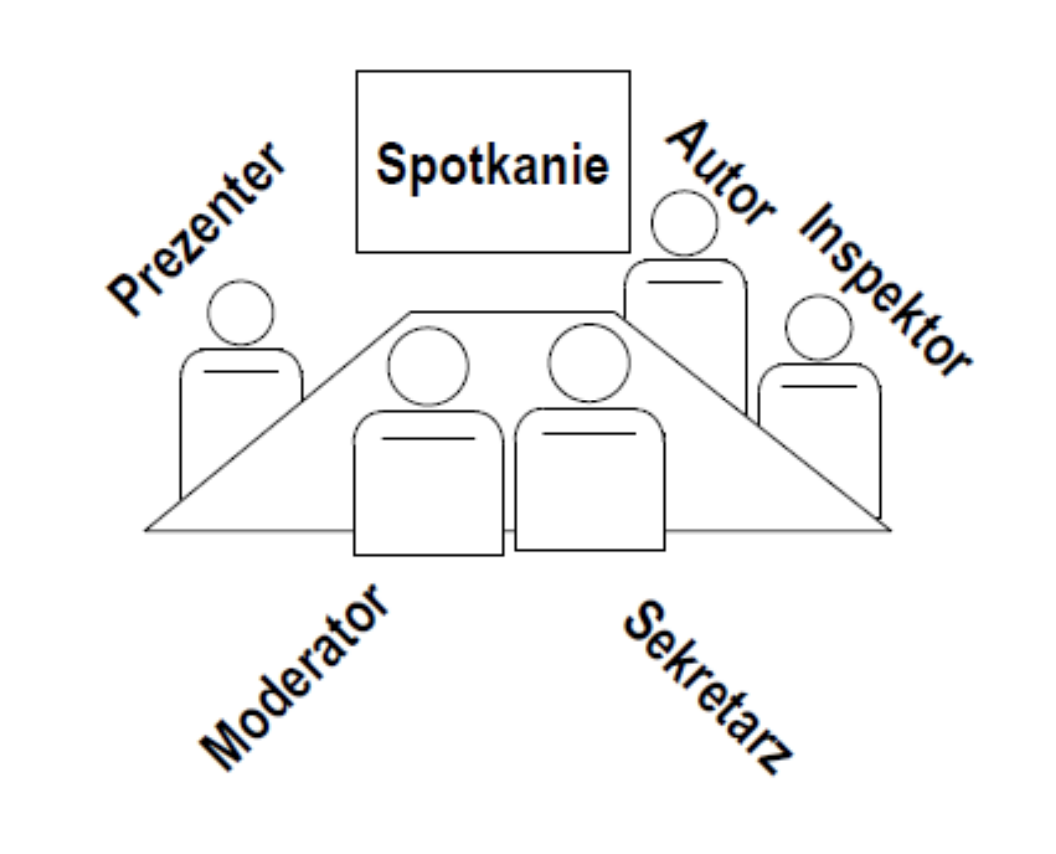
\includegraphics[width=0.5\textwidth]{inspekcja.png}}
                &
                \begin{itemize}
                    \item \textbf{Inspekcja} - ocena artefaktu przeprowadzana przez współpracowników i kierowana przez moderatora
                    \begin{itemize}
                        \item omówienie (cały zespół)
                        \item przygotowaie (indywidualnie)
                        \item inspekcja (cały zespół) - akceptacja pełna lub warunkowa/powtórna inspekcja,
                        \item naprawda
                        \item sprawdzenie
                    \end{itemize}
                \end{itemize}
                \\
            \end{tabular}
        \end{center}
    \end{table}

    \textbf{Inspekcje Fagana}
    \begin{table}[H]
        \begin{center}
            \begin{tabular}{ c c }
                \raisebox{-\totalheight}{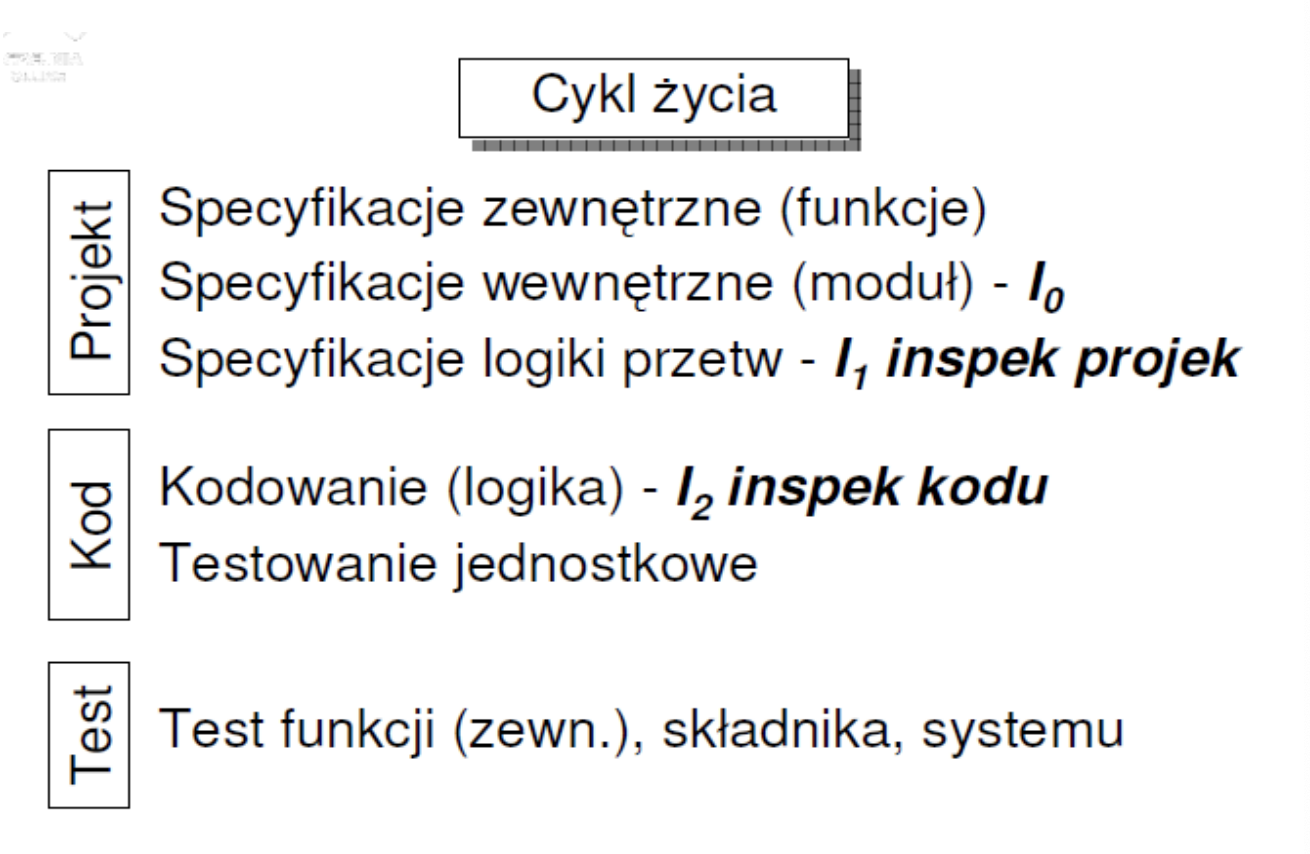
\includegraphics[width=0.5\textwidth]{fag_1.png}}
                &
                \raisebox{-\totalheight}{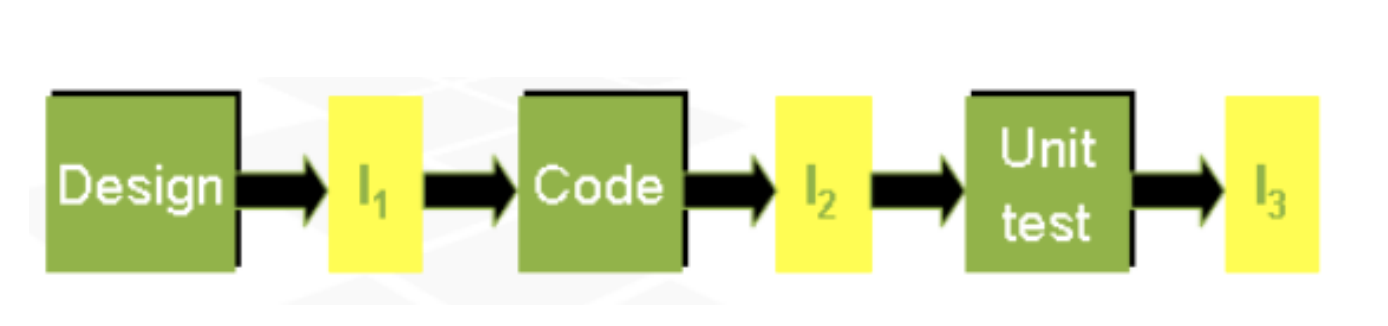
\includegraphics[width=0.5\textwidth]{fag_2.png}}
                \\
            \end{tabular}
        \end{center}
    \end{table}


    \subsubsection{Refaktoryzacja}
    Refaktoryzacja - \textbf{zmiana wewnętrznej struktury programu}, która zwiększa jego \textbf{czytelności} i \textbf{obniża koszt
    pielęgnacji} bez zmiany jego obserwowalnego zachowania.

    \textbf{Motywacja}
    \begin{itemize}
        \item Wysoki koszt pielęgnacji oprogramowania
        \item Naturalny wzrost złożoności i entropii
        oprogramowania
        \item Prawa Lehmana: konieczna ciągła restrukturyzacja
    \end{itemize}

    \hfill \\

    \textbf{Predykat noSideEffectsP}\\
    Wejście:
    \begin{itemize}
        \item Program odwołujący się do zmiennej Var o wartości początkowej 1
        \item Funkcja F potencjalnie modyfikująca wartość Var
    \end{itemize}


    \begin{table}[H]
        \begin{center}
            \begin{tabular}{ p{8cm} p{8cm} }
                \textbf{Problem 1}
                \begin{itemize}
                    \item Czy wywołanie funkcji F powoduje efekt uboczny w
                    postaci zmiany wartości zmiennej Var?
                \end{itemize}
                &
                \textbf{Lemat 1}
                \begin{itemize}
                    \item Problem 1 (braku efektów ubocznych) jest
                    nierozstrzygalny
                \end{itemize}
                \\

                \textbf{Problem 2}
                \begin{itemize}
                    \item Czy istnieje zbiór wejść, który powoduje zmianę
                    wartości zmiennej Var?
                \end{itemize}
                &
                \textbf{Lemat 2}
                \begin{itemize}
                    \item Problem 2 (zmodyfikowany braku efektów
                    ubocznych) jest NP-zupełny.
                \end{itemize}
                \\
            \end{tabular}
        \end{center}
    \end{table}


    \begin{table}[H]
        \begin{center}
            \begin{tabular}{ p{8cm} p{8cm} }
                \textbf{Proste} & \textbf{Trudne}\\
                \toprule
                \begin{itemize}
                    \item zautomatyzowana weryfikacja,
                    \item weryfikowane poprzez statyczną analizę kodu
                    \item można dowieść ich poprawności
                    \item obecnie w wielu środowiskach IDEs
                \end{itemize}
                &
                \begin{itemize}
                    \item weryfikacja wymaga testowania
                    \item testy muszą zostać stworzone ręcznie
                    \item nie można dowieść ich poprawności analitycznie
                    \item wymagają testów jednostkowych
                \end{itemize}
            \end{tabular}
        \end{center}
    \end{table}




\end{document}